\section{Ableitungen}

Regeln:\\
\begin{itemize}
    \item Produktregel: $f'*g+f*g'$
    \item Kettenregel: algemein: $\textcolor{red}{g(}f(x\textcolor{red}{)} = \textcolor{red}{g'(}f(x)\textcolor{red}{)}*f'(x)$\\
          $y=\textcolor{red}{(}x^2\textcolor{red}{)^3} \rightarrow y'=\textcolor{red}{3*(}x^2\textcolor{red}{)^2} \rightarrow y'=6x*(x^2)^2 = 6x^5$
    \item Potenzregel: $y=\sqrt{x} = x^\frac{1}{2} \rightarrow \frac{1}{2}*x^{-\frac{1}{2}} = \frac{1}{2}*\frac{1}{x^\frac{1}{2}} = \frac{1}{2\sqrt{x}}$
\end{itemize}


\hfill \break
\subsection{Graphisches Ableiten}

Zu merken:\\
\begin{itemize}
    \item Das Maximum bzw. Minimum von $f(x)$ wird in der Ableitungsfunktion $f'(x)$ zur Nullstelle.
    \item Der Wendepunkt von $f(x)$ wird in der Ableitungsfunktion $f'(x)$ zum Minnimum und Maximum.
    \item Eine positive Steigung in $f(x)$ beutet positieve Werte in $f'(x)$.
    \item Eine negative Steigung in $f(x)$ beutet negative Werte in $f'(x)$.
    \item Als Sattelpunkt bezeichnet man einen Punkt an dem die Tangente wagrecht ist das bedeutet $f(x) = 0$ und $f"(x) = 0$
    \item Beim Graphischen Ableiten wird der Sattelpunkt zur Extremstelle.
\end{itemize}
\break
\newpage
\subsection{Graphisches Ableiten Beispiele}

\hfill \break
\begin{itemize}
    \item \textcolor{blue}{Funktion}
    \item \textcolor{red}{Ableitung}
\end{itemize}

\hfill \break
Example $f(x) = 2x-1$:\\
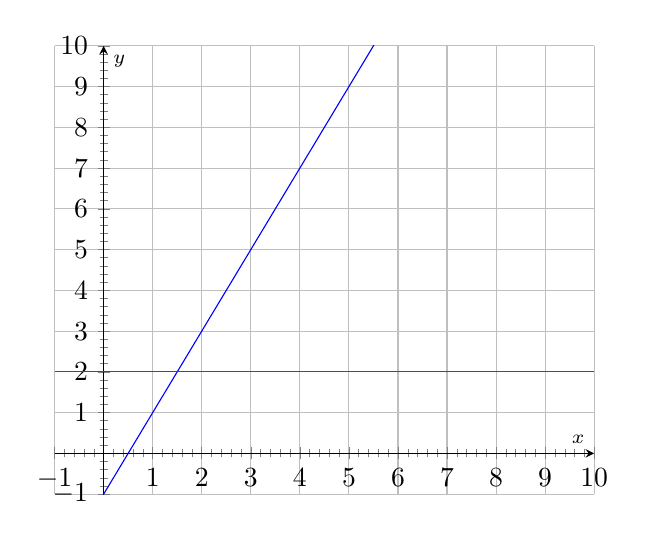
\begin{tikzpicture}[scale=1]
    \begin{axis}%
        [
            grid=major,
            xtick={-1,0,...,10},
            minor x tick num=4,
            xmin=-1,
            xmax=10,
            xlabel={\scriptsize $x$},
            axis x line=middle,
            ytick={-1,0,...,10},
            minor y tick num=4,
            ymin=-1,
            ymax=10,
            ylabel={\scriptsize $y$},
            axis y line=middle,
            no markers,
            samples=100,
            domain=-1:10,
        ]
        \addplot[blue] (x,{2*x-1});
        \addplot[red] (x,{2});
    \end{axis}
\end{tikzpicture}

\hfill \break
Example $f(x) = ((x-1)^2)-1$:\\
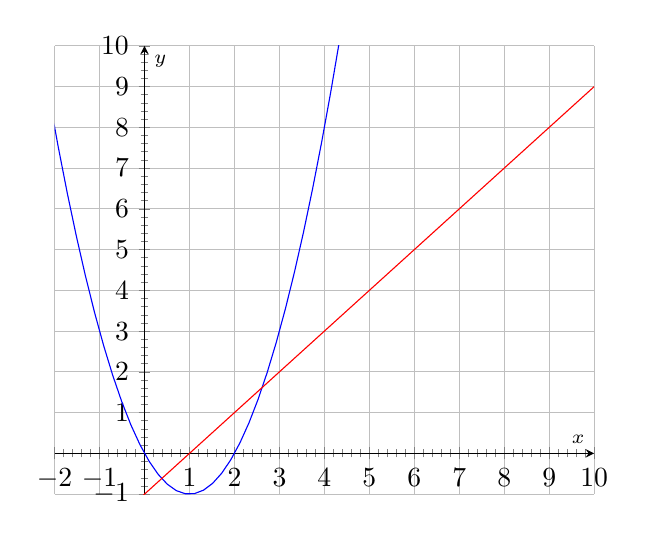
\begin{tikzpicture}[scale=1]
    \begin{axis}%
        [
            grid=major,
            xtick={-2,-1,...,10},
            minor x tick num=4,
            xmin=-2,
            xmax=10,
            xlabel={\scriptsize $x$},
            axis x line=middle,
            ytick={-1,0,...,10},
            minor y tick num=4,
            ymin=-1,
            ymax=10,
            ylabel={\scriptsize $y$},
            axis y line=middle,
            no markers,
            samples=100,
            domain=-10:10,
        ]
        \addplot[blue] (x,{((x-1)^2)-1});
        \addplot[red] (x,{2(x-1)});
    \end{axis}
\end{tikzpicture}
\break
\newpage
\subsection{Funktion Aufstellen}

Eine Parabel, die durch den Koordinatenursprung geht, hat den Scheitel S. Stelle die Gleichung der zugehörigen
quadratischen Funktion auf.\\

Anhaltspunkte:\\
\begin{itemize}
    \item $f(x) = ax^2+bx+c$
    \item $P=(0|0)$
    \item $S=(5|-6)$
    \item $f(0)=0$
    \item $f'(5)=-6$
    \item $f"(5)=0$
\end{itemize}

\begin{align*}
    f'(x) & = 2ax+b \mbox{ // hier die erste ableitung der Basis Funktion } \\
    0     & = 0a+0b+c                                                      \\
    -6    & = 25a+5b+c                                                     \\
    0     & = 10a+b                                                        \\
    f(x)  & = \frac{6}{25}x^2-\frac{12}{5}
\end{align*}
\break
\newpage
\subsection{Musterbeispiel für eine vollständige Kurvendiskussion}

Gegeben ist eine Funktion $f(x)=x^3-3x+1$ Führe eine vollständige Diskussion der Funktion durch.\\

\begin{enumerate}
    \item Die Funktion und ihre Ableitungen: \begin{itemize}
              \item $f(x)=x^3-3x+1$
              \item $f'(x) = 3x^2-3$
              \item $f''(x) = 6x$
          \end{itemize}
    \item Nullstellen ermitteln: $f(x)=0$ \begin{itemize}
              \item $x^3-3x+1=0$
              \item Zur Berechnung gibt es zwei Möglichkeiten mit dem TR: \begin{enumerate}
                        \item grafisch: $y1$ in die Liste eingeben 2nd - calc - zero ; Cursor links und rechts setzen und jeweils  mit ENTER bestätigen.\\ $N_1(-1,88|0)$; $N_2(0.35|0)$; $N_3(1.53|0)$;
                        \item SOLVER: Math - 0 - $\uparrow$ eqn: $0=x^3-3x+1$ ENTER x = Startwert eingeben (-10, 0, 10; auf Verdacht probieren) bzw. eventuell Tabelle 2nd - table nützen 
                    \end{enumerate}
          \end{itemize}
    \item Extremstellen berechnen: \begin{itemize}
        \item $f'(x)=0$
        \item $f''(x) < 0$ = Hochpunkt
        \item $f''(x) > 0$ = Tiefpunkt
        \item $3x^2-3=0$ $\rightarrow$ $3x^2=3$ $\rightarrow$ $x^2=1$ $\rightarrow$ $x = \pm 1$
        \item $f''(-1)<0$ $\rightarrow$ $f(-1)=3$ $\rightarrow$ Hochpunkt $H(-1|3)$
        \item $f''(1)>0$ $\rightarrow$ $f(1)=-1$ $\rightarrow$ Tiefpunkt $T(1|-1)$
    \end{itemize}
    \item Wendepunkt berechnen: $f''(x)=0$ \begin{itemize}
        \item $6x=0$
        \item $x=0$
        \item $f(0)=1$ Wendepunkt $W(0|1)$
    \end{itemize}
    \item Wendetangente berechnen: $t_w:y=kx+d$ \begin{itemize}
        \item $k=f'(0)=-3$
        \item $t_w:y=kx+d$
        \item $W(0|1)$ in y = $-3x+d$ einsetzen 
        \item $1=-3*0+d$
        \item $d=1$
        \item $t_w:y=-3x+1$
    \end{itemize}
\end{enumerate}



\break
\newpage
\subsection{Übersetzungshilfen zum Aufstellen von Gleichungen (Differentialrechnung)}

\begin{itemize}
    \item ... verläuft durch den Punkt $P(2|6)$ $\implies$ $f(2)=6$
    \item ... hat Nullstelle bei $x=9$ $\implies$ $f(9)=0$
    \item ... schneidet die y- Achse bei $3$ $\implies$ $f(0)=3$
    \item ... schneidet die Gerade mit $y=3x-7$ auf der y-Achse $\implies$ $f'(0)=3$
    \item ... berührt die x-Achse an der Stelle $x=5$ $\implies$ $f(5)=0$ und $f'(5)=0$ 
    \item ... hat einen Tiefpunkt bei $T(2|-7)$ $\implies$ $f(2)=-7$ und $f'(2)=0$
    \item ... hat einen Wendepunkt bei $P(-1|2)$ $\implies$ $f(-1)=2$ und $f'(-1)=0$
    \item ... besitzt im Punkt $P(2|-3)$ die Steigung 4 $\implies$ $f(2)=-3$ und $f(2)=4$
    \item ... besitzt an der Stelle $x=-2$ eine Wendetangente mit Steigung 1 $\implies$ $f''(-2)=0$ und $f'(-2)=1$
    \item ... die Tangente in $P(-1|5)$ ist parallel zur Gerade $y=6x$ $\implies$ $f(-1)=5$ und $f(-1)=6$
\end{itemize}
\break
\newpage
\subsection{Ableitung einiger anderen Funktionen}

\begin{itemize}
    \item $f(x)=\frac{1}{5}*(x^3-2x^2+7) \implies f'(x)=\frac{1}{5}*(3x^2)-4x$
    \item $f(x)=x^3*x^5 \implies f(x)=x^8 \implies f'(x)=8x^7$
    \item $f(x)=\frac{sin(x)}{f}*\frac{3x}{g} \implies f'(x)=cos(x)*3x+sin(x)*3$
    \item $f(x)=\frac{cos(x)}{x^2} \implies \frac{f'*g - f*g'}{g^2} \implies f'(x)=\frac{-sin(x)*x^2)-cos(x)*2x}{x^4} = \frac{-sin(x)*x-2*cos(x)}{x^3}$
\end{itemize}